\chapter{Feasibility of Learning}\label{Sec:Feasibility of Learning}

No practical amount of data can distinguish between two distributions, thus instances of GBS can not be proven to come from GESIS. However, machine learning allows to infer the conditional probability of \textit{'GBS participant is representative'} given the survey data within a probabilistic framework. 




\section{Likert-Type Mismatch}

Inconsistencies are discovered later with the planned learning models as 

\begin{figure}[ht]
	\begin{center}
		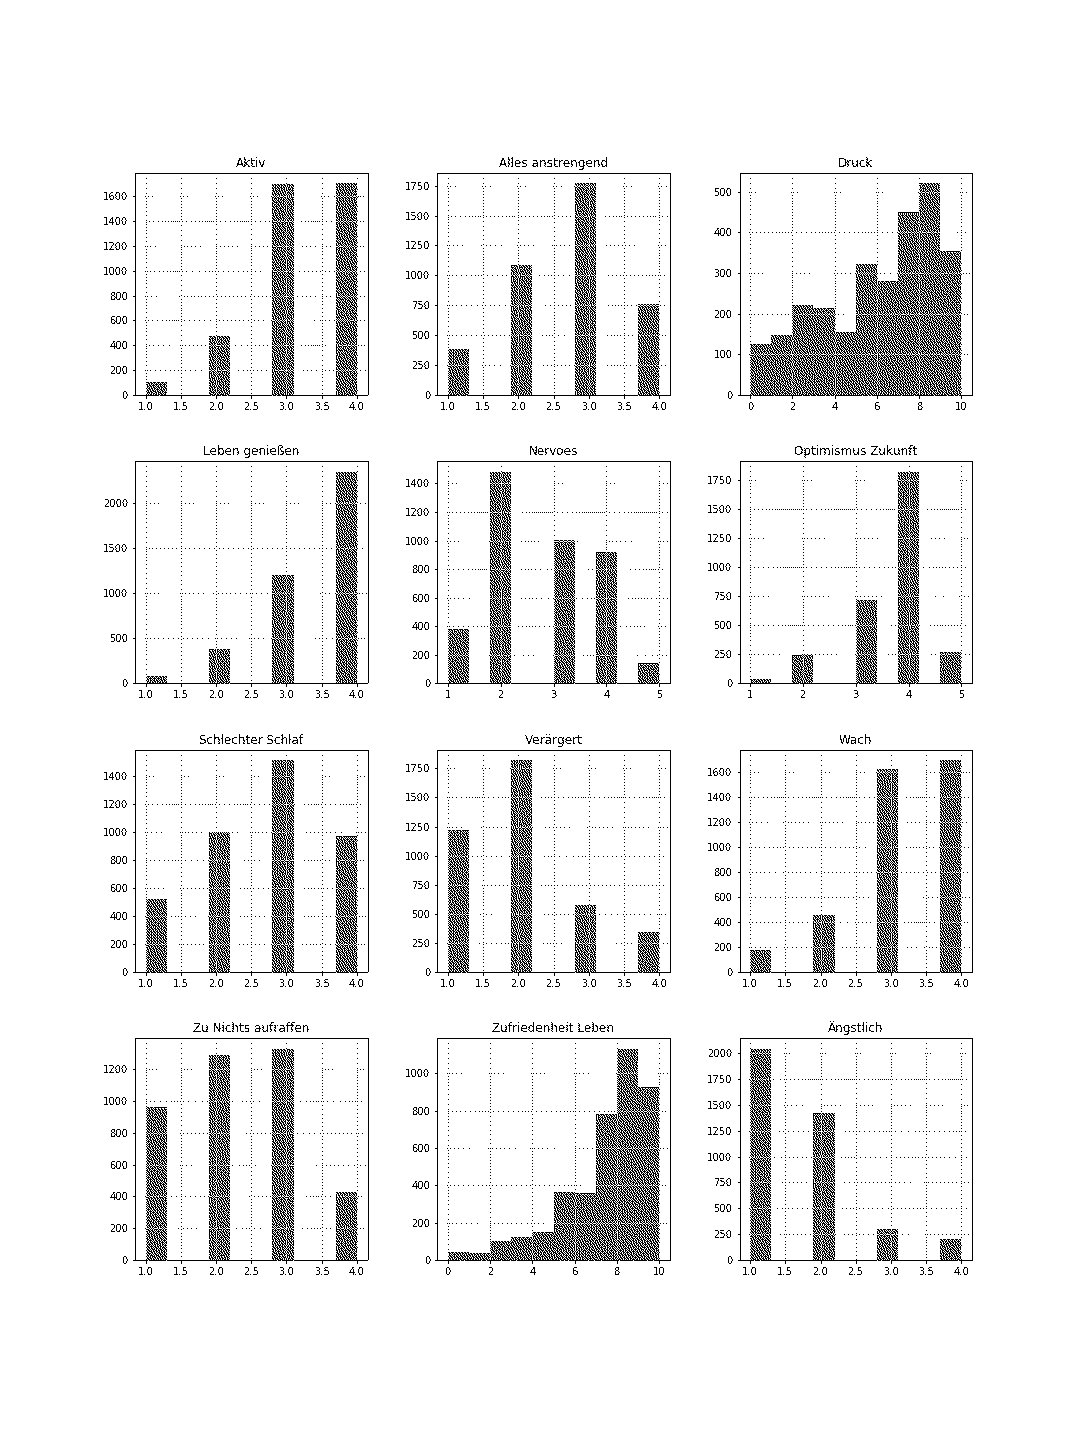
\includegraphics[scale=0.44,angle=0]{fig/gesis_hist}
		\label{std}
		\caption{GESIS hists.}
	\end{center}
\end{figure}

\begin{figure}[ht]
	\begin{center}
		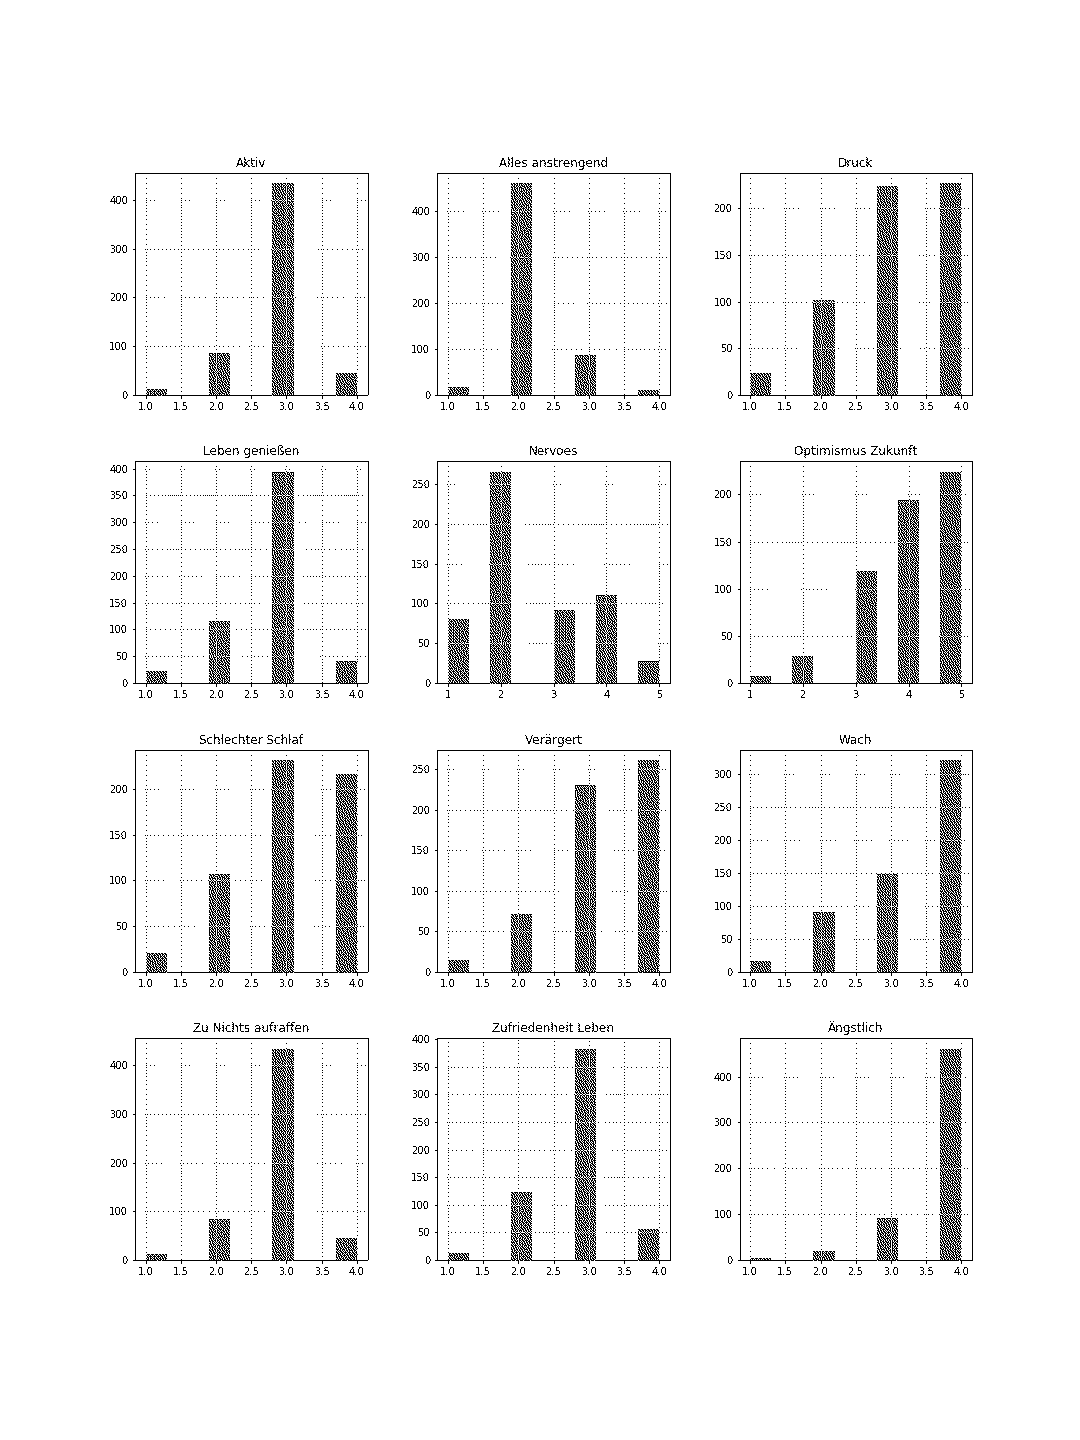
\includegraphics[scale=0.44,angle=0]{fig/gbs_hist}
		\label{std}
		\caption{GBS hists.}
	\end{center}
\end{figure}

John Tukey wrote otherwise (back in 1960) in a monograph "Data Analysis and Behavioral Science" (published in Collected Works v. III). One result he obtained is that if you're getting better than about 10percent test-retest agreement, your scale isn't narrow enough!

[1] It is confirmed that different numbers of rating bars in a subjective rating scale can have significant effects on the subjective measurement, thus the assessment of the Big Five dimensions of personality.

Techniques for reducing the length of scales while maintaining psychometric quality.
Figure X shows an example of such as a statement.

\begin{figure}[ht]
	\begin{center}
		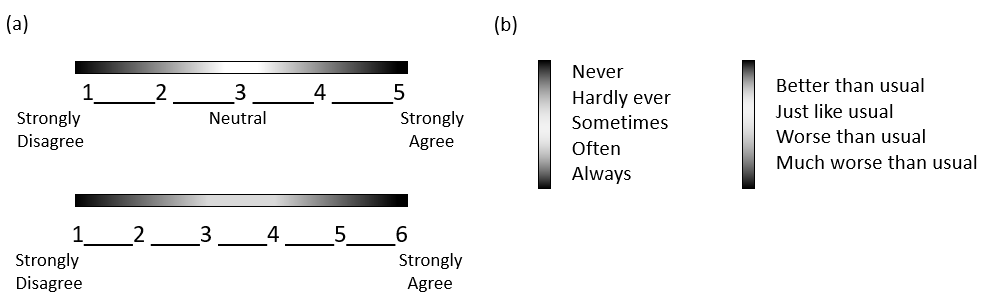
\includegraphics[scale=0.55,angle=0]{fig/scales}
		\label{6_5}
		\caption{Example of a Likert item discrepancy. GBS uses an odd number of responses with a "neutral" option, such as "no opinion", "neither agree nor disagree" or some phrase to that effect. In contrast, there is an even number of responses for this item in GESIS encouraging participants to voice a positive or negative opinion.}
	\end{center}
\end{figure}

In some cases, an additional "opt-out" option is provided for those respondents who truly cannot respond in GBS only.

\begin{table}[ht]
    \begin{center}
            {\footnotesize
            \begin{tabular}{l|c|ccccccccc}
                \hline \hline
		Raw Data & GESIS & 1 & 2 & 3 & 4 & 5 & 6 \\
                     & GBS & 1 & 2 & 3 & 4 & 5 & \\
                \hline
		Max Scaler & GESIS & 0.83 & 1.7 & 2.5 & 3.3 & 4.2 & 5.0 \\
                     & GBS & 1 & 2 & 3 & 4 & 5 & \\
                \hline
		Min-Max Scaler & GESIS & 1 & 1.8 & 2.6 & 3.4 & 4.2 & 5 \\
                     & GBS & 1.0 & 2.25 & 3.5 & 4.75 & 6.0 & \\
                \hline
		Cut-Off Mapping & GESIS & 1 & 2 & 3 & 4 & 5 & 5 \\
                     & GBS & 1 & 2 & 3 & 4 & 5 & \\
            \end{tabular}}
        \caption{Different value scalings of attribute "Desinteresse Politiker".}
\label{Tab:DescripStatsRawData}
\end{center}
\end{table}




\pythonexternal{fig/latex.py}

This leads to a binary classification task with GESIS as positive class and GBS as negative class, i.e. representative and non-representitve sample respectively. Discriminative learners will look for decision boundaries to distinguish the different views of GBS from GESIS in each of the four reference studies. False negatives are then more closely aligned with the target probability distribution. The process of classification is repeated until the learner starts fitting noise more than is warranted. To avoid overfitting, the learning objective needs to be refined as contingency tables lack proper interpretibility. An importance weighted adaption of cross-validation serves as model selection criterion. Given the imbalanced nature and size of GBS, learning is restrained to simpler algorithms with lesser degrees of freedom. The fraction of false positives in the result set of this procedure is kept as proxy measure for the subsequent method positive-unlabeled learning (PU learning). The development of classification models in this setting is often referred to as positive-unlabeled learning (Denis et al. 2005).

\section{Representative Sample}

Some examples include sex, age, education level, socioeconomic status or marital status. Information collections with biased tendencies can't generate a representative sample.

Variables considered in the study must accurately reflect the populations characteristics. 

Consider \textit{attribute: income} of a subset of GBS participants. Statistical significance tests, e.g. Kolmogorov-Smirnov, Chi-Squared

\begin{figure}[ht]
	\begin{center}
		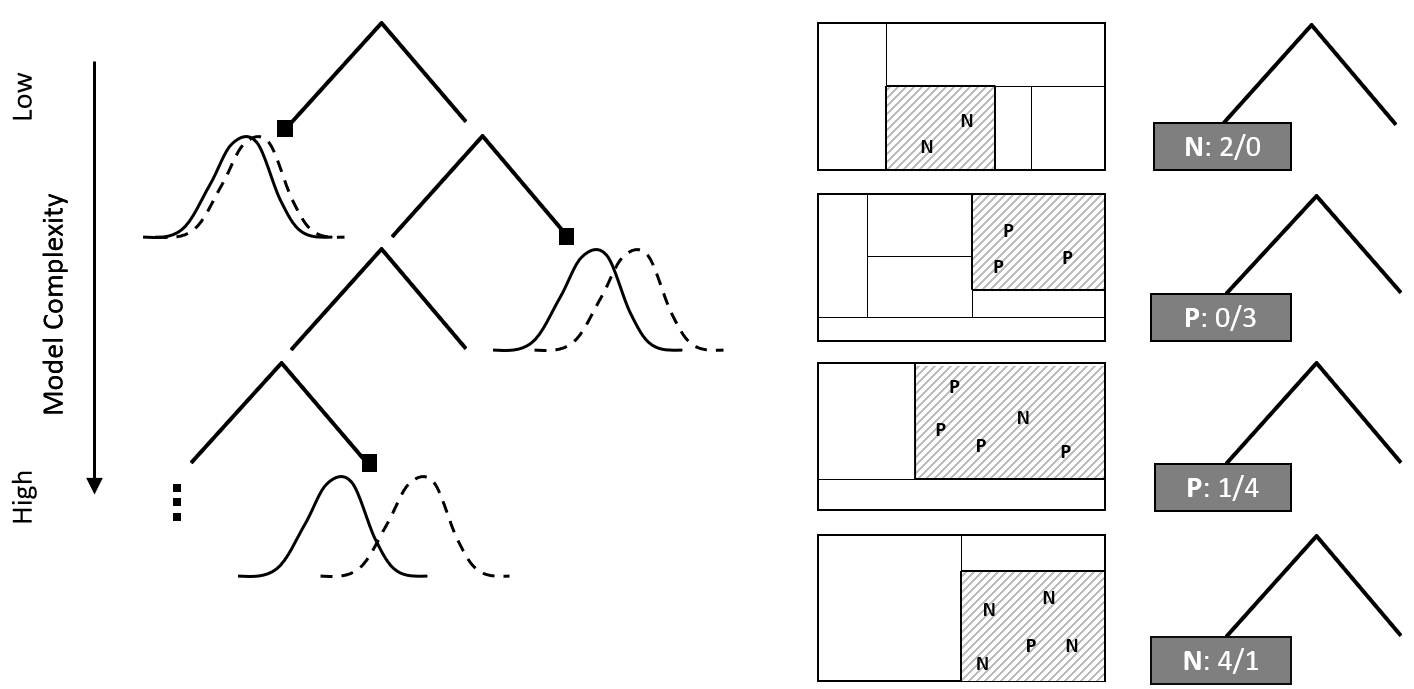
\includegraphics[scale=0.40,angle=0]{fig/tree3}
		\label{project}
		\caption{.}
	\end{center}
\end{figure}

Given a subset of GBS, similarity scores can be defined to evaluate the distance to reference distributions from GESIS. Kolmogorov-Smirnov tests or Chi-Squared assess the likelihood of an attribute of GBS  There are \(2^{|GBS|} = 2^{587}\) subsets of GBS. Evaluating every possible combination of GBS participants and its score is computationally intractable.

A well-defined learning problem where large polls (Umfragedaten) may contain valuable implicit regularities, requires a well-specified task, performance metric and source of training experience [2]. The MRS problem is now stated as a binary classification task with GESIS as positive class and GBS as negative class. Consider designing a computer program to learn to distinguish between . Using prior knowledge together with past experience to guide learning, a machine learning algorithm
is fed with data from games that have been played by chess grandmasters. From this information, the program will learn to apply certain functions to specific board states and make decisions about which move to play next.

Consider a randomly chosen survey participant, i.e. an instance of GBS or GESIS. If the poll indicates the or

Descriptive statistics can be used to 
 
No practical amount of data can distinguish between two distributions, thus instances of GBS can not be proven to come from GESIS. However, discriminative learning allows to infer the conditional probability of \textit{'instance of GBS/GESIS'} given the survey data within a probabilistic framework:

Discriminative learners will look for decision boundaries to distinguish the different views of GBS from GESIS. False negatives are then more closely aligned with the target probability distribution. The process of classification is repeated until the learner starts fitting noise more than is warranted. To avoid overfitting, the learning objective needs to be refined as contingency tables lack proper interpretibility. Given the imbalanced nature and size of GBS, learning is restrained to simpler algorithms with lesser degrees of freedom. The fraction of false positives in the result set of this procedure is kept as proxy measure for the subsequent method positive-unlabeled learning (PU learning). The development of classification models in this setting is often referred to as positive-unlabeled learning (Denis et al. 2005).

\vspace{15pt}
\begin{figure}[ht]
	\begin{center}
		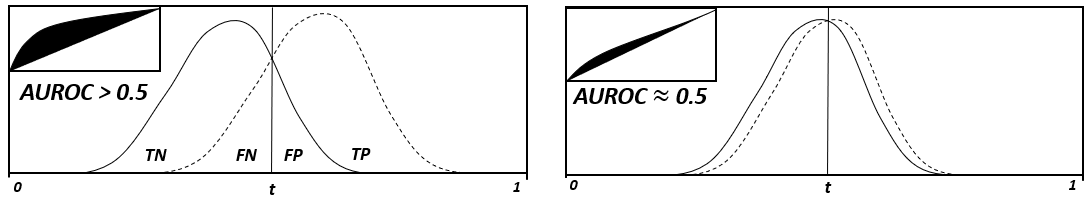
\includegraphics[scale=0.48,angle=0]{fig/roc_example}
		\label{project}
		\caption{There is no caption for such a stupid figure.}
	\end{center}
\end{figure}

PU learning is a semi-supervised technique that does not make the simplifying assumption of GBS instances being negative. Instead, a one-class classifier is trained on GESIS only. [...] This can result in even better assessment. [Read Literature] - Imporance weighted cross validation and pu learning with proper assessment.


PU learning is a semi-supervised technique that does not make the simplifying assumption of GBS instances being negative. Instead, a one-class classifier is trained on GESIS only. [...] This can result in even better assessment. [Read Literature] - Imporance weighted cross validation and pu learning with proper assessment.

%\lstinputlisting[language=Python]{tex_code/test.py}

For further, more technical reading, references to background papers are provided in [38].

Overfitting stands out as one of the biggest challenges for machine learning. It is not exclusive to machine learning but rather a fundamental problem across science and is at the very heart of the dangers of statistical inference. By definition, statistical inference is taking the results of applying some sort of construct or model to specific data and then speculating that it would continue to perform well beyond the original observation range.

State-of-the-art techniques in positive-unlabeled learningtackle this problem by treating the unlabeled sample as neg-atives and training a classifier to distinguish between la-beled (positive) and unlabeled examples. 
Surprisingly,for a variety of performance criteria, non-traditional classi-fiers achieve similar performance under traditional evalua-tion as optimal traditional classifiers (Blanchard et al. 2010;Menon et al. 2015). 

\begin{figure}[ht]
	\begin{center}
		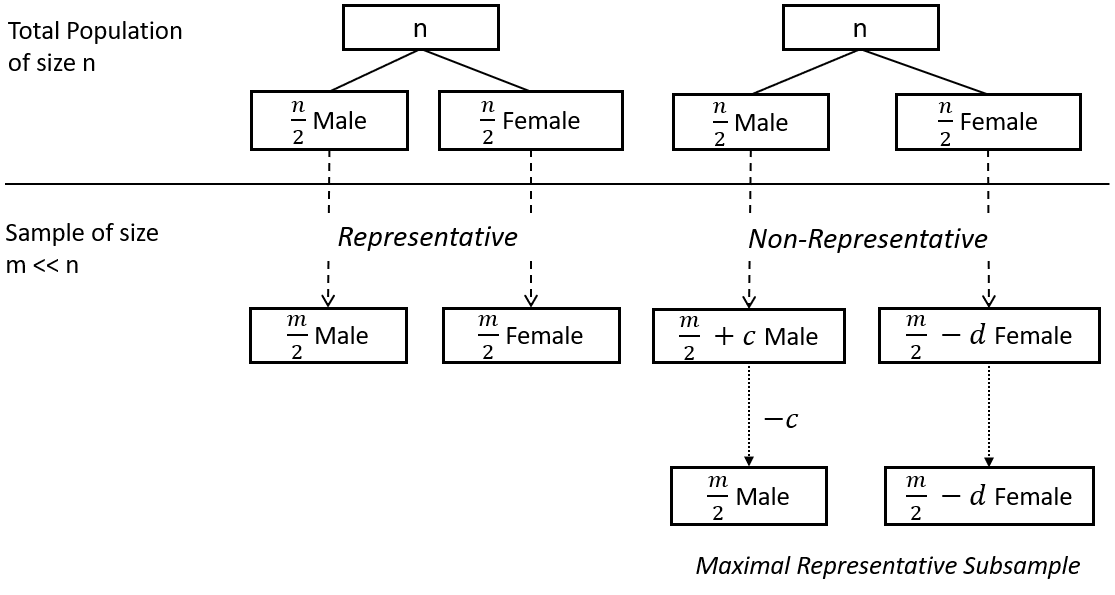
\includegraphics[scale=0.54,angle=0]{fig/Representative}
		\label{representativ}
		\caption{Consider samples of fixed size \(m\) with some constants \(c_m\) and \(d_m\). Maximal representative sampling adjusts for nonresponse \(-d\) of subgroup \(Female\) by removing \(+d\) of subgroup \(Male\) from the sample.}
	\end{center}
\end{figure}

\section{Learning from Positive and Unlabeled Data}

Breiman [9] introduced bagging as a technique to construct strong ensembles by combining a set of base models. Breiman [10] stated that “the essential problem in combining classifiers is growing a suitably diverse ensemble of base classifiers” which can be done in various ways [12]. In bagging, the ensemble models use majority voting to aggregate decisions of base models which are trained on bootstrap resamples of the training set. From a Bayesian point of view, bagging can be interpreted as a Monte Carlo integration over an approximated posterior distribution [40]. 

In his landmark paper, Breiman [9] noted that base model instability is an important factor in the success of bagging which led to the use of inherently instable methods like decision trees in early bagging approaches [19, 11]. The main mechanism of bagging is often said to be variance reduction [4, 10]. In more recent work, Grandvalet [24] explained that base model instability is not related to the intrinsic variability of a predictor but rather to the presence of influential instances in a data set for a given predictor (so-called leverage points).
The effect of bagging is explained as equalizing the influence of all training instances, which is beneficial when highly influential instances are harmful for the predictor’s accuracy.

We have shown the effect of resampling contaminated sets and provided some basic insight into the mechanics of bagging. We will now link these two elements to justify bagging approaches in the context of contaminated training sets. Its usefulness can be considered by both the variance reduction argument of Bauer and Kohavi [4] and equalizing the influence of training points as described by Grandvalet [24]. Variance reduction. Resampling a contaminated set yields different levels of contamination in the resamples as explained in Section 3.1. Varying the contamination between base model training sets induces variability between base models without increasing bias. This observation enables us to create a diverse set of base models by resampling both P and U. The variance reduction of bagging is an excellent mechanism to exploit the variability of base models based on resampling [4, 10]. In the context of RESVM, a tradeoff takes place between increased variability (by training on smaller resamples, see Figure 1) and base models with increased stability (larger training sets for the SVM models). (https://arxiv.org/pdf/1402.3144.pdf)

\hfill \\

\begin{algorithm}[H]
\noindent\rule{12cm}{1.1pt}
\caption{PU training procedure}\label{alg:alg1}
\KwIn{\(P\): set of positive instances (GESIS)}
\myinput{\(U\): set of unlabeled instances (GBS)}
\myinput{\(n_{models}\): number of base models in ensemble}
\myinput{\(n_P\): size of bootstrap sample of \(P\)}
\myinput{\(n_U\): size of bootstrap sample of \(U\)}
\KwResult{Scoring function \(f:U \rightarrow \) $\mathbb{R}$}
\noindent\rule{6cm}{0.4pt}\\
Initualize: 
\(f(x) \leftarrow 0\) and 
\(c(x) \leftarrow 0\)\\
\For{t = 1 to \(n_{models}\)}{
\hfill \\
  Draw a bootstrap sample \(P_t\) of size \(n_P\). \\
  Draw a bootstrap sample \(U_t\) of size \(n_U\). \\
  Train classifier \(f_t\) to discriminate \(P_t\) against \(U_t\). \\
  For any \(x \in U \backslash U_t\), update:
\[f(x) \leftarrow f(x) + f_t(x),\]
\[c(x) \leftarrow c(x) + 1\]
}
Return \[s(x) = f(x)/c(x)\]
\hfill \\

\end{algorithm}

\begin{comment}
\begin{algorithm}[H]
\caption{Transductive bagging PU learning}\label{alg:alg2}
\KwIn{\(P\): set of positive instances (GESIS)}
\myinput{\(U\): set of unlabeled instances (GBS)}
\myinput{\(K_P\): size of bootstrap samples, \(T\): number of base models in ensemble}
\KwResult{Ranking score \(s:U \rightarrow \) $\mathbb{R}$}

\For{t = 1 to \(T\)}{
 Draw a bootstrap sample \(P_t\) of size \(K_P\). \\
 Train classifier \(f_t\) to discriminate \(P_t\) against \(U\). \\
 For any \(x \in U \backslash U_t\), update:
\[f(x) \leftarrow f(x) + f_t(x),\]
\[n(x) \leftarrow n(x) + 1\]
}
Return \[s(x) = f(x)/n(x)\]

\end{algorithm} 
\end {comment}


\subsection{Recovering Model Performance}

\begin{table}[ht] 	
    \begin{center}
            {\footnotesize
            \begin{tabular}{l|cccccccccc}
                \hline \hline
                           &  TP Rate & FP Rate & Precision & Recall & F-Measure & ROC Area & PRC Area & Class \\
                \hline
                      & 0.000 & 0.000 & ? & 0.000 & ? & 0.500 & 0.130 & GBS &\\
                      & 1.000 & 1.000 & 0.870 & 1.000 & 0.931 & 0.500 & 0.870 & GESIS &\\
                \hline \hline
		 W. Avg. & 0.870 & 0.870 & ? & 0.870 & ? & ? & 0.500 & 0.774 &
            \end{tabular}}
        \caption{Some descriptive statistics of location and dispersion for 2100 observed swap rates for the period from February 15, 1999 to March 2, 2007. Swap rates measured as 3.12 (instead of 0.0312). See Table \ref{Tab:DescripStatsRawDataDetail} in the appendix for more details.}
\label{Tab:DescripStatsRawData}
\end{center}
\end{table}

methods to estimate true classificationperformance. 

be recov-ered with the knowledge of class priors

results in biased empirical estimates of the classifier performance
now can be corrected with the knowledge of class priors
using the One-Class SVM and its ability to capture the shape of the data set, hence performing better when the data is strongly non-Gaussian, i.e. with two well-separated clusters;

The ROC curve provides in-sight into trade-offs between the classifier’s accuracies onpositive versus negative examples over a range of decisionthresholds. 
(pr-rc) curve, a plot of precision as a function of recall.The precision-recall evaluation, including summary statis-tics derived from the pr-rc curve, may be preferred to ROCcurves when classes are heavily skewed (Davis and Goad-rich 2006).Although model learning and performance evaluation in asupervised setting are well understood (Hastie et al. 2001),the availability of unlabeled data gives additional optionsand also presents new challenges. A typical semi-supervisedscenario involves the availability of positive, negative and(large quantities of) unlabeled data. Here, the unlabeled datacan be used to improve training (Blum and Mitchell 1998) orunbias the labeled data (Cortes et al. 2008); e.g., to estimateclass proportions that are necessary to calibrate the modeland accurately estimate precision when class balances (butnot class-conditional distributions) in labeled data are notrepresentative (Saerens et al. 2002). This is often the casewhen it is more expensive or difficult to label examples ofone class than the examples of the other. 

The intuition for these results comesfrom the fact that in many practical situations, the posteriordistributions in traditional and non-traditional setting pro-vide the same optimal ranking of data points on a given testsample (Jain et al. 2016; Jain, White, and Radivojac 2016).

Such perfor-mance estimation often involves computing the fraction(s)of correctly and incorrectly classified examples from bothclasses; however, in absence of labeled negatives, the frac-tions computed under the non-traditional evaluation are in-correct, resulting in biased estimates. Figure 1 illustratesthe effect of this bias by showing the traditional and non-traditional ROC curves on a handmade data set. Becausesome of the unlabeled examples in the training set are infact positive, the area under the ROC curve estimated whenthe unlabeled examples were considered negative (non-traditional setting) underestimates the true performance forpositive versus negative classification (traditional setting).This paper formalizes and evaluates performance estima-tion of a non-traditional classifier in the traditional settingwhen the only available training data are (possibly noisy)positive examples and unlabeled data.

Though the efficacy of non-traditional classifiers has beenthoroughly studied (Peng et al. 2003; Elkan and Noto 2008;Ward et al. 2009; Menon et al. 2015), estimating their trueperformance has been much less explored.

the widely-accepted evaluation approaches us-ing ROC or pr-rc curves are insensitive to the variation ofraw prediction scores unless they affect the ranking.

Let \(f\) be the true distribution over the input space \(X\) from which unlabeled data is drawn. With distributions f1 and f0 of the positive and negative examples, respectively, it follows that
\[f(x) = \alpha f_1(x) + (1-\alpha)f_0(x)\]
with positive class prior \(\alpha \in [0,1], x \in X\).

Consider the binary classification problem from input \(x \in X\) (BFI-10 and BRS data) to output \(y \in Y\) (representative: '\(1\)', not representative: '\(0\)'). The learning objective is to discriminate between \(X_p\) drawn according to \(f_1\) and \(X_u\) drawn according to \(f\)  and recover its performance estimate in the traditional setting, i.e. evaluating the decision boundary between positive and negative data.

The two main criteria considered in this work are the area under the ROC curve (AUC) and the F-Measure. The ROC curve plots the true positive rate (recall) of a classifier as a function of its false positive rate (Fawcett 2006) over a range of decision thresholds. 
Furthermore, AUC has a meaningful probabilistic interpretation that is used to  the ability of the classifier to separate classesand is often used to rank classifiers (Hanley and McNeil1982). 
Another important performance criterion generallyused in information retrieval relies on the precision-recall 

 The most extensively studied and widely used performance evaluation in binary classification involves estimating the Receiver Operating Characteristic (ROC) curve t

Recall \(\gamma\), FPR \(\eta\) and Precision \(\rho\) are defined as:

\begin{equation*}
\begin{split}
\gamma = P[\hat{Y} = 1| Y = 1] \\
\eta = P[\hat{Y} = 1| Y = 0] \\
\rho = P[Y = 1| \hat{Y} = 1]
\end{split}
\end{equation*}

where \(\hat{Y}\) is an estimate of the true class label \(Y\).

TPR \(\gamma\) can be estimated directly, because \(X_p\) was sampled from \(f_1\), while this does not hold true for \(\eta\) given the absence of samples from \(f0\).

\begin{gather*}
\gamma = \e{f_1[h(x)]} = \frac{1}{|X_p|} \sum\nolimits_{x \in X_p} h(x) \\
\hat{\eta}^{pu} = \e{f[h(x)]} = \frac{1}{|X|} \sum\nolimits_{x \in X} h(x) \\
\end{gather*}

The area under precision-recall curves \(AUPR\) can be expressed using the approximated value for the fraction of positives \(\alpha\) in \(X_u\)
\[\rho = \frac{\alpha \gamma}{\hat{\eta}^{pu}}\]

The area under ROC curves \(AUROC^{pu}\) so far could only be estimated for the positive versus unlabeled classification by plotting \(\gamma\) and \(\hat{\eta}^{pu}\). To calculate \(AUC\) from \(AUC^{pu}\), S. Jain et al. (2015) express \(\eta\) in terms of \(\hat{\eta}^{pu}\) and \(alpha\) and provide a full derivation from the probabilistic definition of the AUC with

\[\eta = \frac{\hat{\eta}^{pu} - \alpha \gamma}{1 - \alpha}\] so that

\[AUC = \frac{AUC^{pu} - \frac{\alpha}{2}}{1 - \alpha}\] proving

\[AUC > AUC^{pu} \iff AUC^{pu} > \frac{1}{2}\]

TODO: Text here

\subsection{Artificial Data Synthesis}

Thischapterevaluatestheproposedstabilitymeasureandthecorresponding model selection approach by applying it to several synthetic problems and a real-life LGD modeling problem. The experimental setup is as follows. First 

\begin{figure}[ht]
	\begin{center}
		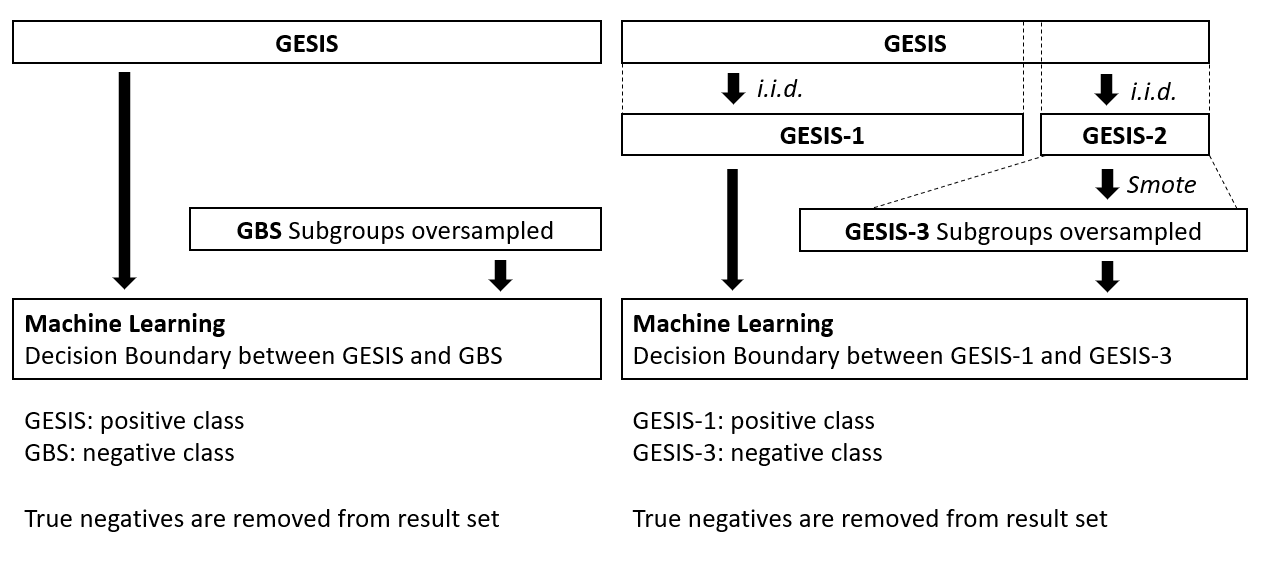
\includegraphics[scale=0.52,angle=0]{fig/procedure}
		\label{std}
	\end{center}
\end{figure}


